\documentclass[14pt]{extbook}
\usepackage{multicol, enumerate, enumitem, hyperref, color, soul, setspace, parskip, fancyhdr} %General Packages
\usepackage{amssymb, amsthm, amsmath, bbm, latexsym, units, mathtools} %Math Packages
\everymath{\displaystyle} %All math in Display Style
% Packages with additional options
\usepackage[headsep=0.5cm,headheight=12pt, left=1 in,right= 1 in,top= 1 in,bottom= 1 in]{geometry}
\usepackage[usenames,dvipsnames]{xcolor}
\usepackage{dashrule}  % Package to use the command below to create lines between items
\newcommand{\litem}[1]{\item#1\hspace*{-1cm}\rule{\textwidth}{0.4pt}}
\pagestyle{fancy}
\lhead{Makeup Progress Quiz -1}
\chead{}
\rhead{Version B}
\lfoot{7547-2949}
\cfoot{}
\rfoot{Fall 2020}
\begin{document}

\begin{enumerate}
\litem{
Solve the linear equation below. Then, choose the interval that contains the solution.\[ \frac{3x -4}{5} - \frac{9x + 9}{2} = \frac{-8x + 3}{4} \]\begin{enumerate}[label=\Alph*.]
\item \( x \in [2, 4.9] \)
\item \( x \in [-4, -2.1] \)
\item \( x \in [-10.7, -6.3] \)
\item \( x \in [1.1, 2.2] \)
\item \( \text{There are no real solutions.} \)

\end{enumerate} }
\litem{
Find the equation of the line described below. Write the linear equation as $ y=mx+b $ and choose the intervals that contain $m$ and $b$.\[ \text{Parallel to } 7 x - 8 y = 5 \text{ and passing through the point } (-10, 7). \]\begin{enumerate}[label=\Alph*.]
\item \( m \in [0.67, 0.92] \hspace*{3mm} b \in [16.8, 19.7] \)
\item \( m \in [-1.04, -0.74] \hspace*{3mm} b \in [-1.8, -0.8] \)
\item \( m \in [1.07, 1.37] \hspace*{3mm} b \in [15.1, 16] \)
\item \( m \in [0.67, 0.92] \hspace*{3mm} b \in [-17.1, -13.3] \)
\item \( m \in [0.67, 0.92] \hspace*{3mm} b \in [15.1, 16] \)

\end{enumerate} }
\litem{
Find the equation of the line described below. Write the linear equation as $ y=mx+b $ and choose the intervals that contain $m$ and $b$.\[ \text{Perpendicular to } 9 x - 7 y = 11 \text{ and passing through the point } (-8, -7). \]\begin{enumerate}[label=\Alph*.]
\item \( m \in [-1.03, 0.46] \hspace*{3mm} b \in [-16.22, -9.22] \)
\item \( m \in [0.23, 1.07] \hspace*{3mm} b \in [-2.78, 0.22] \)
\item \( m \in [-2.02, -1.07] \hspace*{3mm} b \in [-16.22, -9.22] \)
\item \( m \in [-1.03, 0.46] \hspace*{3mm} b \in [1, 6] \)
\item \( m \in [-1.03, 0.46] \hspace*{3mm} b \in [9.22, 15.22] \)

\end{enumerate} }
\litem{
Solve the linear equation below. Then, choose the interval that contains the solution.\[ \frac{7x -9}{6} - \frac{7x + 8}{3} = \frac{-3x -8}{5} \]\begin{enumerate}[label=\Alph*.]
\item \( x \in [4.88, 8.88] \)
\item \( x \in [-6.53, -1.53] \)
\item \( x \in [-0.14, 2.86] \)
\item \( x \in [-17.88, -14.88] \)
\item \( \text{There are no real solutions.} \)

\end{enumerate} }
\litem{
Write the equation of the line in the graph below in Standard form $Ax+By=C$. Then, choose the intervals that contain $A, B, \text{ and } C$.
\begin{center}
    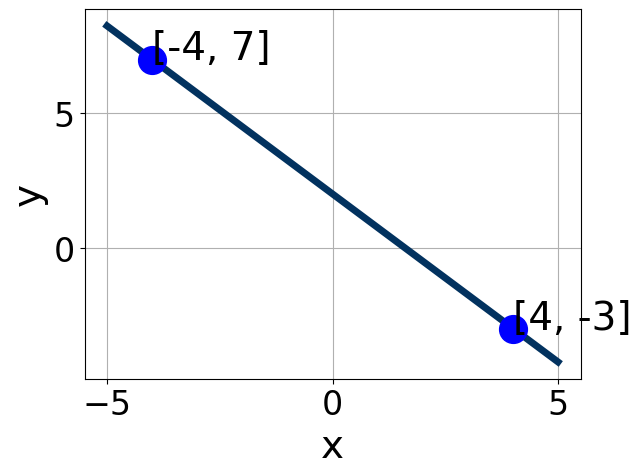
\includegraphics[width=0.5\textwidth]{../Figures/linearGraphToStandardCopyB.png}
\end{center}
\begin{enumerate}[label=\Alph*.]
\item \( A \in [3, 10], \hspace{3mm} B \in [-4.3, -2.9], \text{ and } \hspace{3mm} C \in [-9.9, -4.3] \)
\item \( A \in [1.25, 4.25], \hspace{3mm} B \in [-0.8, 2.1], \text{ and } \hspace{3mm} C \in [1.2, 3.5] \)
\item \( A \in [3, 10], \hspace{3mm} B \in [2.6, 5.3], \text{ and } \hspace{3mm} C \in [7.3, 9.9] \)
\item \( A \in [-5, -3], \hspace{3mm} B \in [-4.3, -2.9], \text{ and } \hspace{3mm} C \in [-9.9, -4.3] \)
\item \( A \in [1.25, 4.25], \hspace{3mm} B \in [-3.3, -0.6], \text{ and } \hspace{3mm} C \in [-2.7, 0.5] \)

\end{enumerate} }
\litem{
Solve the equation below. Then, choose the interval that contains the solution.\[ -15(3x -16) = -19(-17x -8) \]\begin{enumerate}[label=\Alph*.]
\item \( x \in [-1.58, -1.32] \)
\item \( x \in [0.02, 0.64] \)
\item \( x \in [-1.1, -0.89] \)
\item \( x \in [0.73, 1.42] \)
\item \( \text{There are no real solutions.} \)

\end{enumerate} }
\litem{
Solve the equation below. Then, choose the interval that contains the solution.\[ -18(-6x + 11) = -12(-19x -2) \]\begin{enumerate}[label=\Alph*.]
\item \( x \in [1.09, 1.96] \)
\item \( x \in [0.46, 0.62] \)
\item \( x \in [-1.64, -0.94] \)
\item \( x \in [-2.12, -1.66] \)
\item \( \text{There are no real solutions.} \)

\end{enumerate} }
\litem{
First, find the equation of the line containing the two points below. Then, write the equation as $ y=mx+b $ and choose the intervals that contain $m$ and $b$.\[ (-6, 6) \text{ and } (-8, 2) \]\begin{enumerate}[label=\Alph*.]
\item \( m \in [1, 7] \hspace*{3mm} b \in [11.59, 12.12] \)
\item \( m \in [1, 7] \hspace*{3mm} b \in [16.79, 18.46] \)
\item \( m \in [1, 7] \hspace*{3mm} b \in [-20.7, -17.61] \)
\item \( m \in [1, 7] \hspace*{3mm} b \in [7.87, 11.51] \)
\item \( m \in [-5, 0] \hspace*{3mm} b \in [-15.99, -13.79] \)

\end{enumerate} }
\litem{
First, find the equation of the line containing the two points below. Then, write the equation as $ y=mx+b $ and choose the intervals that contain $m$ and $b$.\[ (9, -3) \text{ and } (11, 6) \]\begin{enumerate}[label=\Alph*.]
\item \( m \in [0.5, 7.5] \hspace*{3mm} b \in [-7, -1] \)
\item \( m \in [-6.5, -2.5] \hspace*{3mm} b \in [52.5, 57.5] \)
\item \( m \in [0.5, 7.5] \hspace*{3mm} b \in [-48.5, -39.5] \)
\item \( m \in [0.5, 7.5] \hspace*{3mm} b \in [42.5, 46.5] \)
\item \( m \in [0.5, 7.5] \hspace*{3mm} b \in [-14, -11] \)

\end{enumerate} }
\litem{
Write the equation of the line in the graph below in Standard form $Ax+By=C$. Then, choose the intervals that contain $A, B, \text{ and } C$.
\begin{center}
    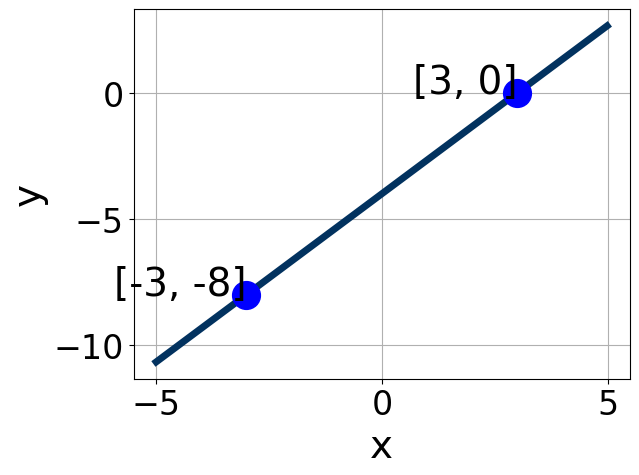
\includegraphics[width=0.5\textwidth]{../Figures/linearGraphToStandardB.png}
\end{center}
\begin{enumerate}[label=\Alph*.]
\item \( A \in [-2.33, -0.33], \hspace{3mm} B \in [0.68, 1.03], \text{ and } \hspace{3mm} C \in [-6, -3] \)
\item \( A \in [2, 9], \hspace{3mm} B \in [-3.81, -2.52], \text{ and } \hspace{3mm} C \in [12, 15] \)
\item \( A \in [-5, -2], \hspace{3mm} B \in [2.91, 3.7], \text{ and } \hspace{3mm} C \in [-14, -6] \)
\item \( A \in [-2.33, -0.33], \hspace{3mm} B \in [-2.01, 0.22], \text{ and } \hspace{3mm} C \in [4, 7] \)
\item \( A \in [2, 9], \hspace{3mm} B \in [2.91, 3.7], \text{ and } \hspace{3mm} C \in [-14, -6] \)

\end{enumerate} }
\end{enumerate}

\end{document}